\section{能源的开发和利用}\label{sec:5-7}

机器的运转,汽车的行驶,火车的开动,飞机的飞行……都要消耗一定的能量。
就是做饭、照明、取暖等日常生活也都要消耗能量。凡是能够提供能量的东西都可以叫做能源。
煤、石油和天然气在燃烧时放出大量的热能,它们就是能源。
流动的水和空气可以推动水轮机和风力发动机工作,它们也是能源。

\begin{figure}[htbp]
    \centering
    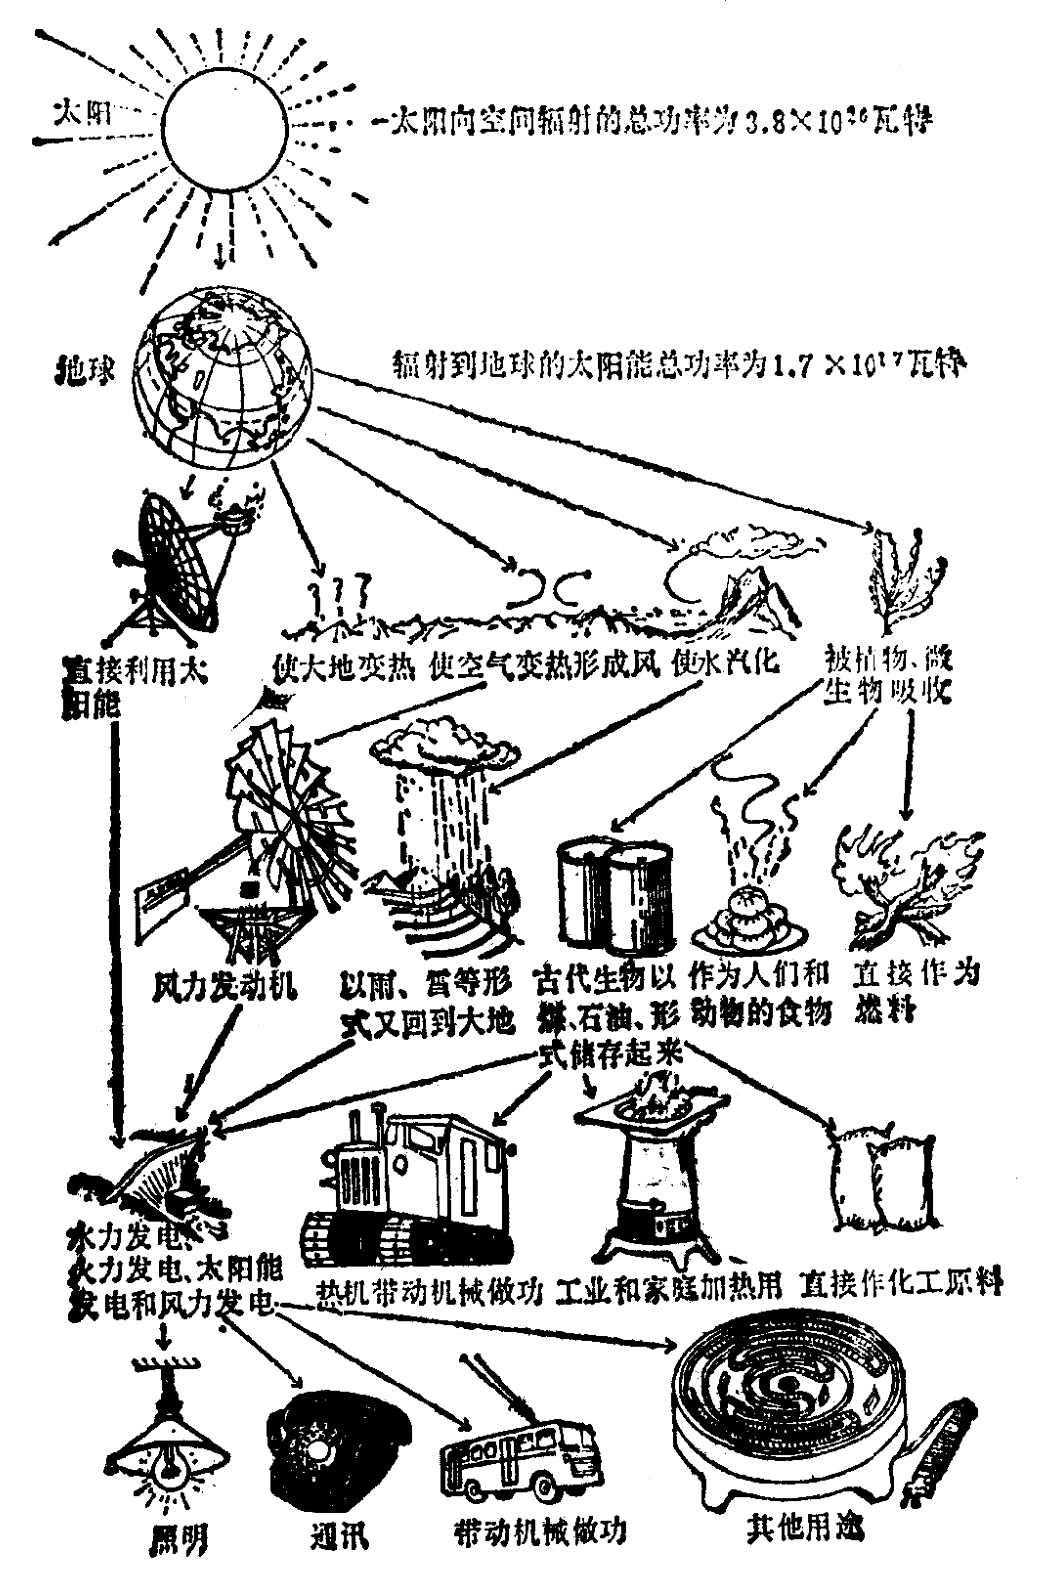
\includegraphics[width=0.7\textwidth]{../pic/czwl2-ch5-7}
    \caption{太阳能的利用示意图}\label{fig:5-7}
\end{figure}

随着科学技术的发展,人类开发和利用能源的范围不断扩大。
但是,到目前为止,人类社会使用的仍然主要是煤、石油和天然气。
现代的生产和生活中能量的消耗愈来愈大,近些年来更有急剧上升的趋势。
煤、石油和天然气等的贮量总是有限的,不可能无限制地满足人们不断增长的需要。
这就是近年来人们常常谈到的能源危机。为了解决这个问题,我们要不断地探索能的转化的新途径,
有效地利用已经探明的能源,努力开发和利用新的能源。

新的能源中,当前人们最为瞩目的是原子能。
原子核发生变化时释放的能量叫做原子能,也叫核能。
人们对原子能的利用从四十年代开始到现在已经有了巨大的发展,已经可以建立核电站生产大量的电能。
目前,我国也正在筹建功率很大的核电站。

太阳发出的光和热具有能,它是一个十分巨大的天然能源。
据计算,到达地面的太阳能的总量大约是地球上目前正在为人类利用的各种能源的总功率的一、两万倍。

人类利用煤、石油和天然气的能量,利用水能和风能,归根到底都是间接利用太阳能,
因为它们都是来源于太阳的光和热(图 \ref{fig:5-7})。
直接利用太阳能的比较简便的方法是把太阳能转化为热能,如在第一章介绍的太阳灶和太阳炉。
在温度要求不太高的情况下,还可以采用吸热式集热箱来获得太阳能。
集热箱实际上是一个开有透明窗口、内壁涂黑的保温箱。
保温箱的构造如图 \ref{fig:5-8} 所示,在太阳照射下,箱内的温度可以超过一百度。
(这种集热箱能够使箱内温度升高的道理,可以根据你学过的热学知识来解释。)
利用太阳能获得的热能,可以用来产生水蒸气(或热气),再利用水蒸气(或热气)膨胀带动机器作功,
如带动水泵的太阳能水泵,带动汽轮发电机组的太阳能发电。
还可以直接利用太阳能发电,第七章介绍的硅光电池,就是直接利用太阳能获得电能的。

\begin{figure}[htbp]
    \centering
    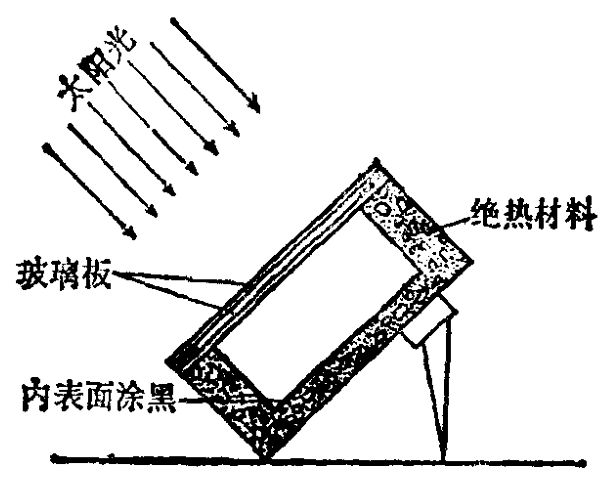
\includegraphics[width=0.4\textwidth]{../pic/czwl2-ch5-8}
    \caption{}\label{fig:5-8}
\end{figure}

太阳能具有取之不尽、用之不竭、清洁无污染等优点。
因此,太阳能的利用引起了各国的重视,有着广阔的发展前途。
可以预料,到二十一世纪,太阳能将是人们利用的主要能源之一。

我国是能源比较丰富的国家。已经探明,我国煤的储藏量达 6000 亿吨,居世界第三位,
石油的储藏量居世界第八位,核能原料也十分丰富。
解放以来我国能源开发的增长速度是比较快的。
解放后三十年,全国能源生产总量增长了 26 倍。
但是,随着现代化建设的发展和人民生活水平的提高,对能源的需要也将不断增长。
因此,我国也在大力研究能源的合理开发问题。

为了适应现代化建设对能源的需要,在抓好能源开发的同时,还必须注意能源节约。
目前我国在能源的生产、运输、转化、使用等方面都存在很大浪费,主要原因有技术陈旧、设备落后、管理不善等。
为了节能,需要采取多种措施,例如,采取先进的能耗小的工艺流程,进行以节能为中心的技术改造,
以省煤、省油、效率高的锅炉、热机、电机等设备替换陈旧落后的设备,规定各种产品和用能设备的能耗标准,
制定能源使用中的奖惩制度,等等。
我们每个同学,不但自己要注意节能,还应该注意宣传节能的意义,这也是对祖国社会主义现代化建设的贡献。


\lianxi

(1) 1 焦耳的热能,可以使 10 克水的温度升高多少度?

(2) 一壶 5 千克的水,温度从 20 ℃ 升高到 100 ℃,吸收的热量是多少卡?相当于多少焦耳?

用这些功来把你举高,可以把你举多高?

(3) 1 千克汽油完全燃烧放出的热量是多少焦耳?

(4) 举几个常见的热能和机械能相互转化的例子。

